\documentclass[tikz,border=10pt]{standalone}
\usepackage{amsmath}

\begin{document}
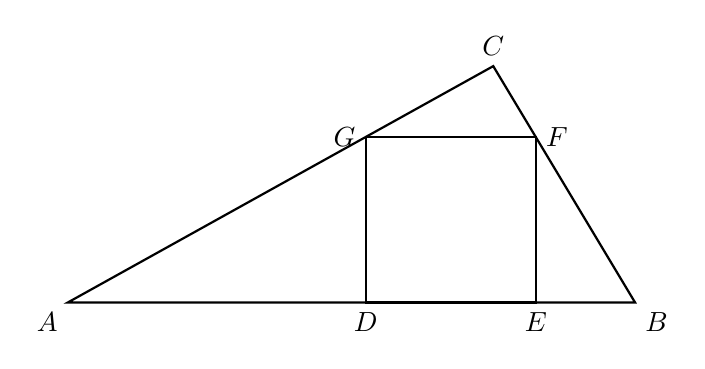
\begin{tikzpicture}[>=stealth, thick, scale=1.2]

    % 1. 定义三角形的基本顶点坐标 (可根据需要调整比例)
    \coordinate (A) at (0,0);
    \coordinate (B) at (6,0);
    \coordinate (C) at (4.5,2.5);

    % 2. 绘制大三角形 ABC
    \draw (A) -- (B) -- (C) -- cycle;

    % 3. 计算内接正方形/矩形的坐标
    % 为了保证 G 在 AC 上，F 在 BC 上，且 DEFG 为矩形，此处设定高度 h
    % 也可以基于相似三角形比例计算，这里采用视觉还原的坐标点：
    \coordinate (G) at (3.15, 1.75); % 位于 AC 边上
    \coordinate (D) at (3.15, 0);    % G 在 AB 上的投影
    
    % 根据平行关系计算 F 点 (F 必须在 BC 线上且高度与 G 相同)
    % 经过计算或交点捕捉确认 F 点
    \coordinate (F) at (4.95, 1.75); 
    \coordinate (E) at (4.95, 0);    % F 在 AB 上的投影

    % 4. 绘制内接矩形 DEFG
    \draw (D) -- (G) -- (F) -- (E) -- cycle;

    % 5. 标注顶点标签
    % anchor 用于微调文字位置，避免覆盖线条
    \node [below left] at (A) {$A$};
    \node [below right] at (B) {$B$};
    \node [above] at (C) {$C$};
    \node [below] at (D) {$D$};
    \node [below] at (E) {$E$};
    \node [right] at (F) {$F$};
    \node [left] at (G) {$G$};

\end{tikzpicture}
\end{document}